\documentclass[11pt,dvipdfm]{article}
%\documentclass[11pt]{article}

\usepackage{deauthor,times,graphicx}

%\graphicspath{{Davidson/}} %uncomment when combining all papers together



\newcommand{\eat}[1]{}

\newcommand{\grid}{{\tt DbD}}

\begin{document}

\title{Disposal by Design}
\author{
  Susan B. Davidson\\
  \small{University of Pennsylvania}\\
  \texttt{\small{susan@cis.upenn.edu}}
  \and
  Shay Gershtein\\
  \small{Tel Aviv University}\\
  \texttt{\small{shayg1@mail.tau.ac.il}}
  \and
  Tova Milo\\
  \small{Tel Aviv University}\\
  \texttt{\small{milo@cs.tau.ac.il}}
  \and
  Slava Novgorodov\\
  \small{eBay Research}\\
  \texttt{\small{snovgorodov@ebay.com}}  
}


\maketitle

\begin{abstract}
The flood of data that has enabled breakthroughs in medicine, commerce, transportation, science and society also threatens to overwhelm our storage capacities and our privacy.  Due to the volume of data and growth of regulations governing its maintenance and use, it is essential to develop automatic disposal techniques to manage this flood.
We present a vision for automating data disposal -- disposal by design -- which takes into account processing constraints, regulatory constraints as well as storage
constraints, and give three concrete examples which address aspects of this vision.  Two of the examples address current needs in e-commerce, while the third suggests how to use machine learning to find summaries of relational data. We then discuss the research challenges that remain to provide a holistic solution to disposal by design.
\end{abstract}




\section{Introduction}
\label{sec: intro}
We are experiencing an amazing data-centered
revolution in almost every aspect of our lives. Huge amounts of
data are being generated, collected, transformed, integrated and
analyzed, leading to breakthroughs in medicine, commerce,
transportation, science and society. This data-centered revolution
is fueled by the massive amount of data that is constantly being generated, and at the same time is threatened by the very same information flood. First, the size of our digital universe is growing exponentially, and it is estimated that, despite continuous advances in storage technology, the demand for storage will outstrip storage production {\em by an order of magnitude} by as early as 2025 \cite{dataage}.
If we do not learn how to effectively dispense with some of this data we will drown. 
Second, uncontrolled data collection endangers security and privacy, as recognized, e.g., by the recent EU Data Protection Regulation (GDPR) \cite{gdpr}. 

This problem has become even greater following the growth of COVID-19 data that has been collected and distributed. Data disposal policies must be systematically developed and enforced to benefit and protect organizations and individuals. 
Due to the volume of data involved and the growth of regulations/policies governing its maintenance and use, it is essential to develop automatic data disposal techniques that take these policies into account to control the information flood.  



A primary advantage of automating data disposal is the ability to focus resources on legitimate, valuable information, thereby enabling the creation of new products and solutions. 
The potential for cost-savings associated with reduced data volumes also provides an attractive solution to companies with tight budgets who cannot afford to store and maintain unlimited data. Furthermore, effective enforcement of data retention, deletion and privacy regulations allows legal and business requirements to be met.


However, it is obviously not enough to consider just policies when disposing of data:  business processes must also be guaranteed to have the data or information available at the level of detail that they need. This leads to the use of ideas such as data sketching and summarization, if the data cannot be outright deleted. However, data  sketching and summarization techniques have only been developed for specific aspects of the problem, mostly related to query answering over structured data \cite{apq,streaming,summerization,compression,amnesia}.  We are still very far from a comprehensive solution that covers the entire data analysis pipeline (e.g. data cleaning, integration, sharing, and analysis, in addition to querying) and the breadth of data types (e.g. images and text, in addition to structured data). Every single data disposal solution therefore has to address, almost from scratch, the same tough challenges. Furthermore, these ad hoc solutions, even when successful, are application specific and rarely shareable.

Retaining the information hidden in the data while respecting storage,  processing, and regulatory constraints is a therefore a major challenge. 
The difficulty stems from the separate, detailed requirements that each of these type of constraints entails. For instance,
satisfaction of {\em processing constraints} is essentially an optimization
problem where one needs to determine what data may be discarded and which summary of it to retain, if needed, so that data utilization is minimally harmed. In contrast, {\em regulatory constraints} tell us what information must be deleted (or kept for a specific time period \cite{WikipediaRetentionPolicy}), and the
challenge is to identify and discard (or retain) all the relevant data. 


To pave the road for sustainable big data management, in this paper we set forth a research vision for automating data disposal which takes into account processing constraints, regulatory constraints, as well as storage constraints which we call {\em disposal by design}.  
To accomplish this vision, 
we must develop the formal scientific foundations for massive-scale data disposal. This encompasses the development of a formal model that captures all the diverse facets of data disposal: retention constraints, heterogeneous data, and data processing pipelines.  It means developing reasoning capabilities over the data processing pipelines to ensure that they work over the retained, possibly summarized, data, and that this can be done in a dynamic manner as retention constraints, data, and pipelines are added, deleted or modified. Such a principled approach is essential for developing reusable solutions, and thereby sustaining the data-centered revolution that is transforming our lives.

We start in Section~\ref{sec: vision} by giving an  architecture for our envisioned disposal by design (\grid) framework.  In Section~\ref{sec: ex} we give three concrete examples which address subproblems of this framework in the context of e-commerce, image and relational data.  We summarize some of the research challenges in Section~\ref{sec: challenges}, and conclude in Section~\ref{sec: concl}.





\section{Vision}
\label{sec: vision}


The architecture of our envisioned framework is shown in Figure~\ref{fig: arch}.
\grid\ takes as initial input a set of {\em constraints}, \textit{C};
a set of heterogeneous data sets \textit{D};
and a set of data analysis pipelines, \textit{A}. 
The constraints include data that must be retained (e.g. photos that must appear on a product page due to licensing agreements, or bank records that must be retained for five year), data that can or must be removed (e.g. due to GDPR regulations or bank records that are older than five years), as well as overall space constraints.  The data is heterogeneous, and includes tables, images, text, etc.  It is annotated with provenance, size and a notion of accuracy.  The analysis pipelines could be ML packages, code, queries, workflows, etc, and are annotated with accuracy constraints on their input data. 
Note that the inputs to the analysis pipelines could be descriptive rather than prescriptive, i.e. there could be choices of different data (of various quality) that could be used as an input.

\newpage
The optimization goal used by \grid\ is some function of space and accuracy.  One example of an optimization goal is to meet some overall space constraint while trying to satisfy the accuracy constraints of the data analysis pipelines.  Another example is to guarantee that the accuracy constraints are satisfied and minimize the overall space.


\begin{figure}
\begin{center}
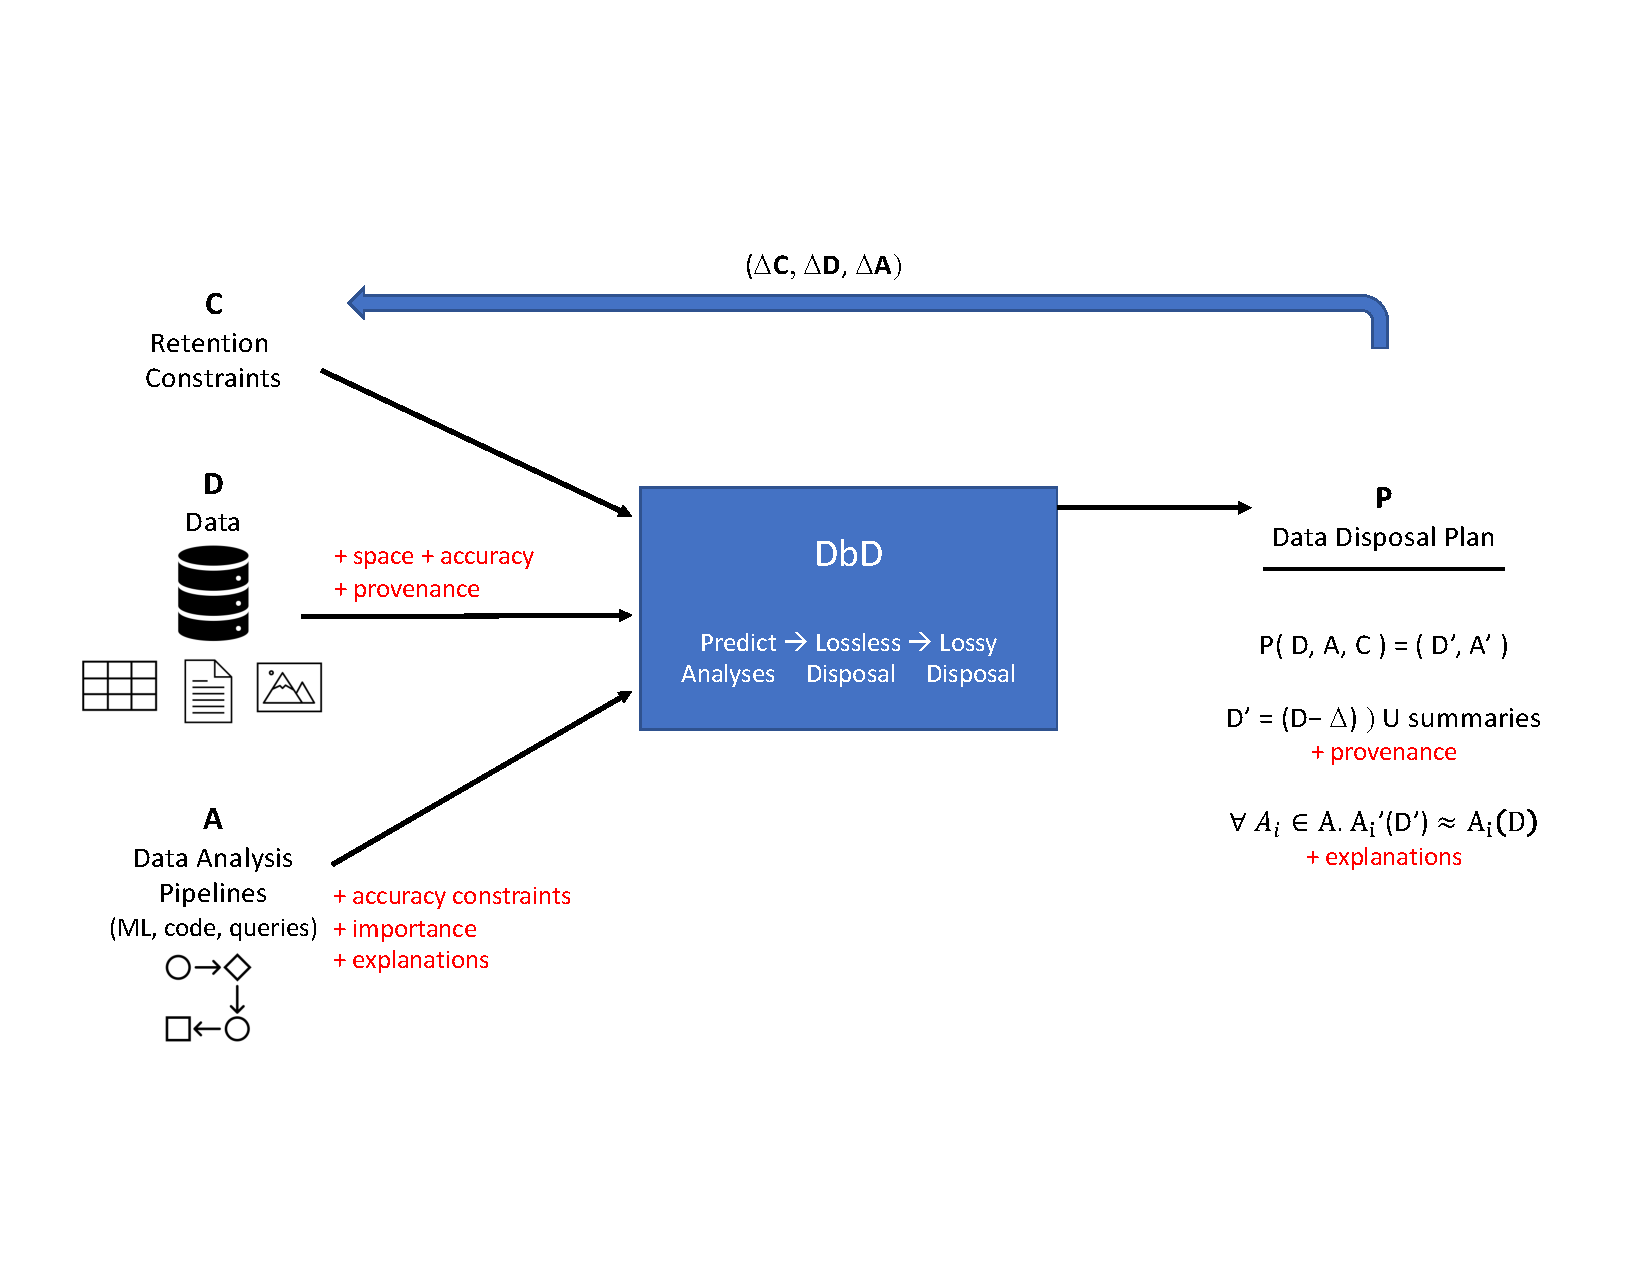
\includegraphics[width=0.8\textwidth, bb = 0 0 820 580]{figs/DbD-arch.pdf}
\vspace{-5mm}
\caption{Architecture of \grid}
\label{fig: arch}
\vspace{-5mm}
\end{center}
\end{figure}


In meeting the optimization goal within \grid, several strategies could be considered: First, attempting to predict future analyses and data usage to avoid disposing of data that might be needed in the future (see, e.g. \cite{MiloS20,sigmod20,ElMS20b}).  Second, discarding any {\em unnecessary} redundant data that is not needed for any potential analysis pipelines or required by retention constraints.  Similarly, unnecessary analysis pipelines that are not required by retention constraints and have not been used for a sufficiently long time could be discarded. We call this a ``lossless'' disposal since it disposes of data/analyses that are not needed.  Third, making harder decisions about how to decrease the quality of potentially {\em necessary} data while still ensuring that the accuracy constraints on data analysis pipelines are met.  We call this a ``lossy" disposal since \mbox{it degrades the quality of data and analyses.}
  
The output of \grid\ is a 
data disposal plan, which includes 
a modified set of data sets, \textit{D'}, in which some data have been removed ($\Delta$) and possibly replaced by less accurate (but smaller) summaries, and a modified set of analysis pipelines, 
\textit{A'}, in which some may have been removed,  modified (e.g. to work over lower accuracy data), or added (e.g. in anticipation of future analysis needs).  The output must guarantee that 1) the retention constraints~\textit{C} are met, and 2) the accuracy of the files of the data set is sufficient to meet the accuracy constraints on the data analysis pipelines.  The output should also able to provide explanations, e.g. for how summaries were obtained and how they meet the accuracy requirements of relevant data analysis pipelines. Since retention constraints, data sets, and data analysis pipelines may be changed, added or removed over time, \grid\ must adaptively recompute over these changes (indicated by the loop back).




\section{Examples of Specialized Instances}
\label{sec: ex}

We mentioned in the introduction that there has been a lot of work on specific aspects of data disposal.  In this section, we highlight two examples from e-commerce that deal with identifying a (bounded size) subset of items of highest utility, out of a large set of items: the first considers a catalog of items for sale~\cite{EDBT20} and the second deals with image data~\cite{SIGMOD-demo}.  In these two cases, the focus is on (a non-traditional form of) data and the workloads are very simple (essentially, select queries).  They also highlight how the inputs to \grid\ can be efficiently computed rather than by relying on humans. Interestingly, the setting in these two works is such that the non-selected items/images are not necessarily disposed off but may rather be stored, e.g., in a secondary storage. Nevertheless the algorithms are oblivious to whether or not a copy of the non-selected items is retained somewhere, and can be employed in both scenarios.


The third example that we present in this section illustrates some work in progress which focuses on (more traditional) relational data and (more complex) aggregate queries, and suggests a less traditional approach to summarization using deep learning.  

\subsection{E-Commerce Catalog Reduction}
\label{ssec: inventory}

Many e-commerce platforms, such as eBay, serve as an intermediary between companies and consumers, receiving a commission per purchase. To increase sales, these platforms tend to offer as many items as possible. However, in many situations a reduced subset of the items should be offered for sale, e.g., when opening an express delivery branch, starting operations in a new region, or disposing of redundant items to improve data quality and decrease maintenance costs.
In all these cases, it is imperative to select a reduced inventory that maximally covers consumer needs. In this problem (which we formalized in \cite{EDBT20}), given a large set of items (\textit{D}), a bound on the number of items that can be retained (\textit{C}), and consumer preferences in terms of items popularity and suitability as alternatives (\textit{A}), the goal is to select a reduced inventory that maximizes the likelihood of a purchase (that is formalized exactly based on A). 

 A na\"{i}ve, yet popular, solution is to focus on the top-selling items. This however ignores the hidden relations between items and, in particular, the tendency of shoppers to buy, in the absence of an item they are looking for, a satisfying alternative. 
Instead, this problem can be modeled via a dedicated weighted directed graph, where the nodes are the items, their weights are the item's popularity (which is calculated based on provenance, i.e. the navigation patterns in the e-commerce platform website), and the weighted edges model to what extent an item may serve as a substitute for another (this can also be derived using provenance, via a statistical analysis of consumer data and purchase records that are available to all e-commerce platforms.).
One can prove that this problem is NP-hard. Moreover, since in practical settings the overall number of items and the bound on the reduced item set are very large - in the order of magnitude of millions - a highly scalable algorithm is needed. 

To solve this problem, we provide in \cite{EDBT20} a highly parallelizable and scalable algorithm, that leverages our graph-based formulation of the problem, along with optimal approximation guarantees.  Moreover, we have developed an end-to-end solution that fits the real-world e-commerce application and provide an extensive set of experiments demonstrating the efficiency and effectiveness of our solution. 

Importantly, the model we defined for this problem is abstract and can be used to capture different use-cases outside of e-commerce settings. 
Each such application, however, requires a different method to derive the input. Specifically, one needs to assign a relative importance score to each item in the inventory, and to quantify the extent to which an item can serve as an alternative for another item. 



\subsection{Archiving Images in E-commerce}
\label{ssec: photos}

We now discuss an example of automating image selection that we are developing in collaboration with eBay, which is being tested for use in their product catalogs~\cite{SIGMOD-demo}. 

eBay has a huge archive of images of products some of which are used for display throughout a hierarchy of landing pages of product categories. For each page, there is a pre-defined subset of images that are relevant for the product category, out of which 
a small set are displayed.  
Each image may be relevant for a large number of different pages, and its value may differ between pages. 
Some of the images are required to appear on certain pages due to legal contracts (a {\em retention constraint}).  Finally, the landing pages themselves may vary in importance, reflecting the relative popularity of product categories.
To speed up the page display, it is desirable to maintain a smaller size image repository (which may be viewed as a bounded-size, fast-access cash), much smaller than the size of the full archive.  The optimization problem is to find a ``good" set of images that can fit in the bounded-size repository (cache) and meet the content and policy requirements of each of the landing pages.

In this application, \textit{C} are simple constraints which state that some set of images must appear on landing pages due to legal contracts, as well as the size of the cache.  
\textit{D} is the set of all photos in the archive; size and provenance are metadata associated with each photo.
\textit{A} represents the set of landing pages, each of which has a title (e.g., ``Nike red shirts'', ``Samsung smartphones'' or ``shoes'').  A landing page can be thought of as a simple query which identifies the set of all photos in the archive that could be used on the page. 

Importantly, information associated with \textit{D} and \textit{A} can be automatically obtained.
For each landing page, the relevance (accuracy) of an image for the page can be computed based both on the quality of the image (we are currently using an internal eBay ML model \cite{dagan2021image}) and the relevance score of the product represented in the image (which can be calculated using the product title and search engine retrieval score).
The relative importance of a landing page can be calculated based on the landing page popularity, i.e. the number of visits in the last 90 days, normalized by sum of all visits to all pages.

An important property in evaluating the quality (goodness) of a solution is the diversity of the set of photos displayed on each page. Therefore, the quality of a solution for this application is not only assessed by the relevance of each individual image to its assigned landing pages, but also using more collective assessments on the subset of images, ensuring that each subset covers the spectrum of products and product aspects relevant for the page. 
To this end, we use a notion of {\em similarity} between photos, which can be calculated using cosine similarity between image embeddings. 
The score of a solution for each landing page is then not only computed based on the relevance scores of the selected subset, but is also based on the similarity of the most similar selected photo to each non-selected photo. This ensures that the selected subset is representative of the entire set of relevant photos, which naturally maximizes diversity and minimizes redundancies.  
The objective function then becomes the weighted sum of the scores for each landing page, where the weights are the relative importances of the pages as discussed above. 

It can be shown that a solution to this problem cannot be approximated beyond a $(1-1/e)$ factor, unless $P=NP$, via a straightforward reduction from the Maximum Coverage problem. We nevertheless give in ~\cite{SIGMOD-demo} an efficient algorithm with a tight worst-case approximation guarantee,
based on the fact that the objective function can be proven to be nonnegative, monotone and submodular, and using an extension of the standard iterative greedy algorithm given in~\cite{sviridenko2004note}. 



We have evaluated our image archival solution within eBay on several product categories (separately, as each category is assigned different analysts and has its own space constraint). Initial reports indicate that our solution significantly reduces manual work; the business analysts reported performing only a small number of modifications to the suggested solution, taking much less time than creating the solution from scratch.





\subsection{Sampling and Aggregating Relational Data}
\label{ssec: reldata}

In the first two examples, the core of the solution is based a formal definition of a problem with an algorithmic solution.  However, another increasingly common approach to solving problems is based on machine learning.  We therefore give a simple example using relational data and aggregate queries, and show how to ``learn" the best subset of data/metadata to store. Note that this is very much work in progress, based on recent work in ~\cite{Mosaic,EntropyDB,Themis}.

Given a set of relational data and  input queries, the goal of our problem is to learn a subset of the data/metadata to store that takes significantly less space, such that it is still possible to compute, based on the retained information, approximate answers to an expected workload of queries with reasonable approximation errors.

In terms of the form of the retained data, we use a common approach: the retained information is a combination of (1) a uniform sample of the original data and (2) aggregates (i.e., results or partial results of aggregate selection queries) computed over the complete original data.
There are several recent works proposing methods for deriving the best approximate answer to a query, given a sample and the aggregates (e.g., \cite{Mosaic, Themis, peng2018aqp++, liang2021combining}). Our focus, however, is on deciding, given an upper bound on the total space used by the retained data, how much of it should be used for each type of data (i.e., the sample or the aggregates), and which aggregates should be stored. Note that we do not need to decide which subset of the data should be stored in the sample, as it is a random uniform sample and the only relevant parameter is therefore its size. 
\label{sec: example}
\begin{figure}
\begin{center}
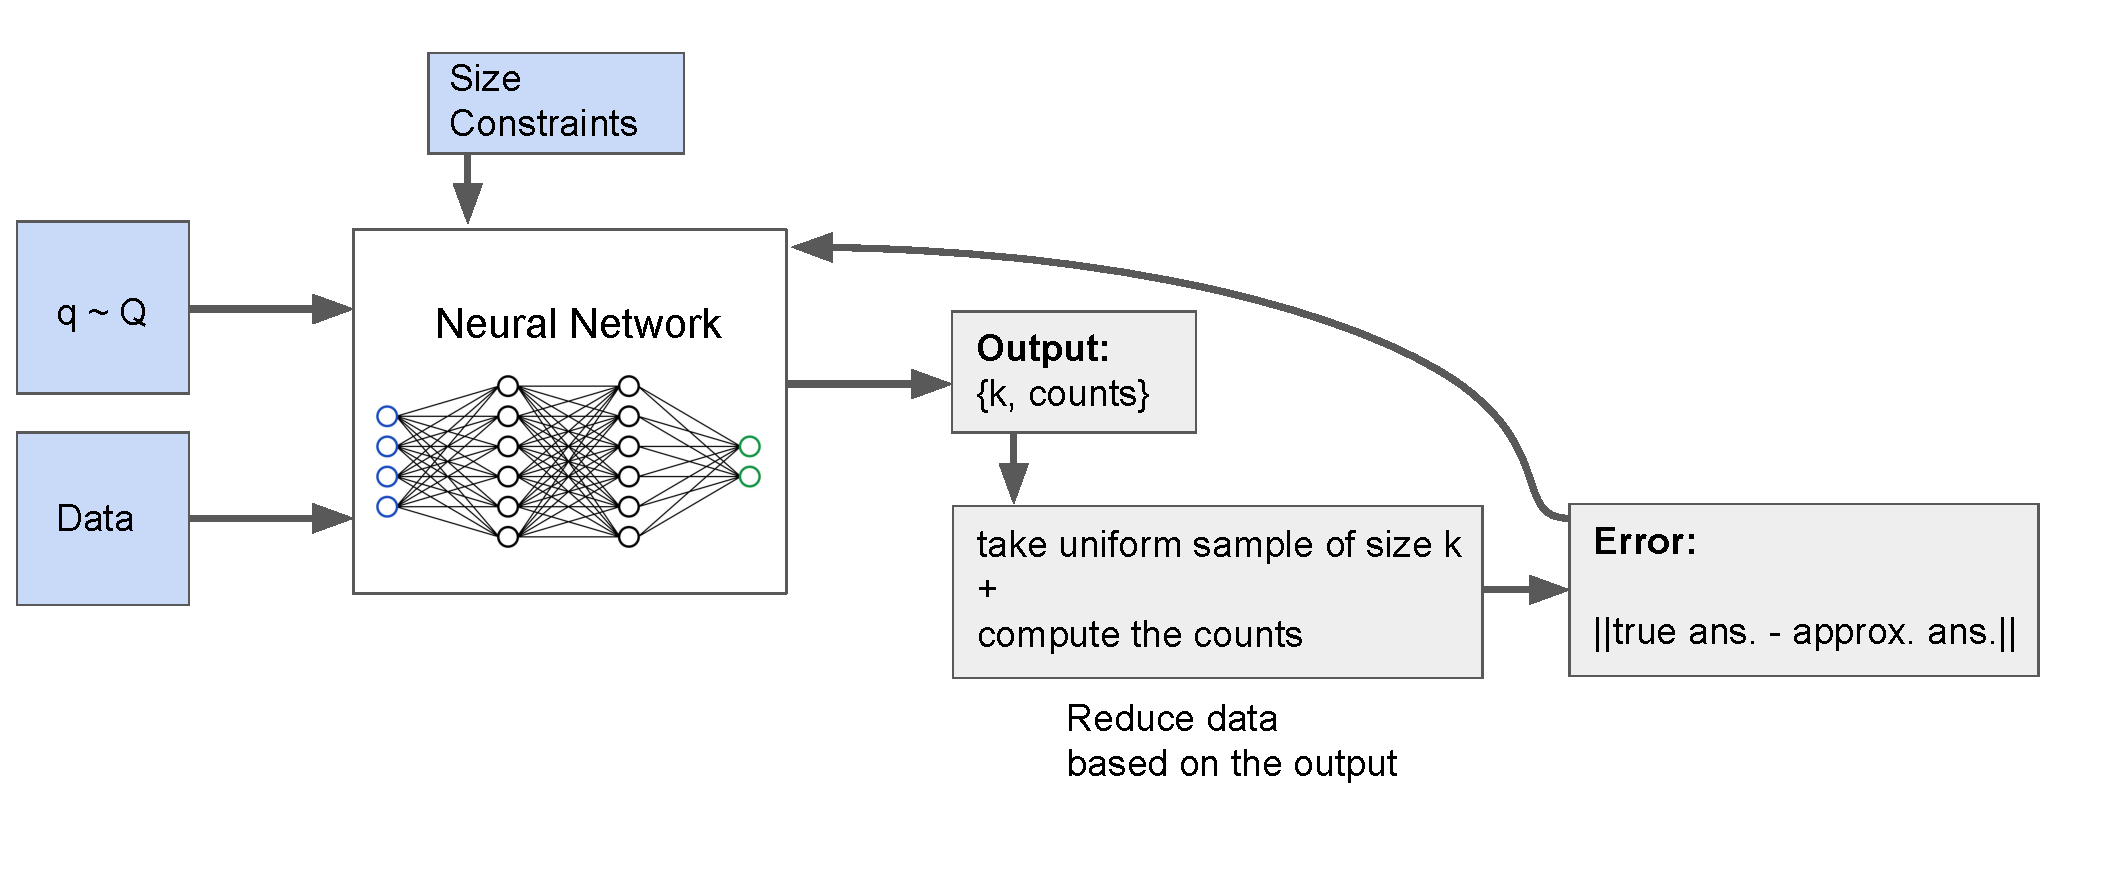
\includegraphics[width=0.95\textwidth, bb = 0 0 1020 424]{figs/example_fig.pdf}
\vspace{-5mm}
\caption{Architecture for learning the best subset of data/metadata to store}
%, based on a distribution \textit{Q} of query workload}
\label{fig: example}
\vspace{-8mm}
\end{center}
\end{figure}

To this end,  we build a model for deriving a distribution \textit{Q} on the expected queries by leveraging query workload information. This is achieved by a GAN-based solution \cite{creswell2018generative}, where you train a generator to produce artificial queries and a discriminator to distinguish between these queries and queries taken from a real-world query workload. The final distribution learned by the generator is \textit{Q}.  

We propose the following architecture, depicted in Figure \ref{fig: example}, that is based on a deep learning approach: a learning model (neural network) receives as input  the data, the space constraint (both are given in the initial setting), and a subset of sample queries generated over \textit{Q}  (these three components of the input to the network correspond to the three blue boxes in the figure). Given this input, the network then produces the size of the uniform sample, and the specific aggregates one should store (the box in the figure marked with the ``Output'' label). Given any such produced solution, the specified aggregates and a uniform sample of the specified size are aggregated, and their utility is evaluated by the resulting approximation errors on a large sample of queries (also sampled from \textit{Q}). 
Note that the methods for computing the approximate answer uses only the reduced data. 
The model learns over time to minimize these errors, as marked by the back-arrow pointing from the ``Error'' box to the network. We note that the format of the output of the network (i.e. a sample along with a set of aggregates) is the same as the format of the input in the recent work of \cite{Themis} for deriving approximate query answers over incomplete databases, and we also use the same evaluation methods for assessing the overall accuracy of the approximate answers (the query answers derived from the partial data) as used in their empirical analysis.


\section{Research Challenges}
\label{sec: challenges}
While the examples in the previous section address specific aspects of disposal by design, we are still far from providing a holistic solution. 
In particular, the examples do not capture the complexity of workloads, variety of data, and dynamic aspects of a full solution.  Thus in more complex settings, a solution would need to be redesigned from scratch.  Therefore we argue that to solve the problem in a principled way, two scientific challenges must be addresses:  designing a unified model, and dynamic incremental computation.
We discuss each of these below, along with the enabling technologies that may be helpful.

\subsection{A Unified Model}
\label{ssec: model}

In order to develop a comprehensive solution to data disposal rather than a series of one-off solutions, we need a unified formal model for all types of data disposal. 
A prime motivation for using a unified model is that it will allow us to consider data sharing and replication between applications, as well as to re-use solutions between applications.  
As illustrated in Section~\ref{sec: vision},
central to the model are notions of data coverage and quality, data usage and workload, storage and
regulatory constraints, and evolution (of data, analysis pipelines  and retention policies) over time.

Furthermore, we believe that the framework should be {\em declarative}. To understand the benefit of a declarative framework, consider the origins of modern relational database management systems \cite{codd70}.
A relational database is essentially a First-Order Logic machine which manages data. More precisely, a
non-specialist can specify some needs declaratively, in first-order
logic terms. The system then compiles such a ``logical query" into
an ``algebraic query plan" that is optimized and evaluated.
Relational systems thus perform automatic reasoning to handle
queries and views, e.g., to rewrite queries into equivalent ones for
optimization. Reasoning is also present in many other aspects of
relational DBs, e.g., dependencies (logical formulas over the data
that the system should enforce) and triggers \mbox{(i.e. active
rules).} In relational systems, such reasoning is in some sense
``hard-wired". For instance, several algebraic query plans may be
possible for a given logical query. The system is in charge of
verifying that the plans considered are indeed equivalent to the
original query. To do that, the system assumes some laws governing
the interaction of operations and implements an algorithm (some
reasoning) to check that these laws are not violated. The laws are
decided in advance and the reasoning is encoded in algorithms whose
correctness has been proven in advance (e.g., the commutativity of joins).

Similarly, we want an intelligent interface between the data and its
disposal process. For data disposal, logic is needed to reason about how 
data relates to analysis tasks, to describe data disposal
and retention constraints and preferences/criteria (the equivalent
to the ``hard-wired" logic of relational systems) and to model
analysis workloads and properties of data summaries.  The laws governing data coverage and
quality, data usage and workload, storage and regulation
constraints, and evolution (of data and retention policies) over
time must therefore be ``first-class citizens'' of the model rather than
inflexible, preconceived laws  (see, e.g., ~\cite{DBLP:conf/ithings/SarkarBRM18}).
Furthermore, the reasoning behind data disposal must be able to take into account the specific context and application domain.


Two key enabling technologies may be helpful in developing this unifying model:  data provenance, and sketching and summarization.

\vspace{-2mm}

\paragraph*{Data Provenance}
Provenance traces the source
of information and the computational process it undergoes, and is
critical for understanding data usage, for explaining query results
and for assessing their validity \cite{prov,moreprov}. In our
setting, provenance must further capture what data has been omitted
and what kind of summary was retained for it. Such
meta-data will allow for effective computation over the
retained information and for explanation/justification of the
obtained results. It will also allow the system to keep a record of the processing
activities, as required by regulations such as GDPR \cite{gdpr}.

\newpage
Attaching provenance to individual data items is typically
straightforward; what is more complex and needs to be studied
is what provenance should be used to annotate
summarized or omitted  data. The difficulty stems from the fact that
common provenance models often apply only to a fairly restricted set
of declarative data manipulation operators (e.g. SQL) whereas data
summarization/deletion strategies are typically given as general
programs, possibly empowered by machine learning (ML) tools
\cite{summerization,amnesia}, for which provenance is not yet well
defined. A second, related, difficulty is to propagate such
meta-data through the analysis process, which may be complex.
Finally, an additional challenge is that the size of provenance may be very large \cite{selprov,provesize}, and so effective
disposal must be recursively applied to this meta-data as well.

\vspace{-2mm}

\paragraph*{Sketching and Summarization}
Much of the data that we keep around is redundant and can be
discarded with no harm. 
Common examples are old document drafts and ancient emails dealing with non important issues. 
But in general,
whether or not data should be kept, and at what level of granularity,
depends on the expected analysis workload.
(as well as the regulatory constraints). 
For a simple example, the analysis could compare multiple versions of the same document, in
which case discarding old (legitimate) versions of documents without
retaining some record of the changes between documents is harmful.
A key challenge thus is
to dynamically determine which data should/may be discarded and, if
allowed, what summary should be kept for the deleted items, so that
data utilization is minimally harmed. 

Traditional techniques for data summarization, sketching and
statistical/approximate query processing are mostly concerned with
specific {\em query} operations and provide {\em accuracy guarantees
w.r.t query answers}. But modern data analysis pipelines are far
more complex, consisting of multiple analysis steps, including data
integration, cleaning, restructuring, visualization, and machine
learning (ML) \cite{bigdatajag}. 
Naturally, it would be desirable to build on existing technology
when possible. 
For instance, in stream data
processing, incoming data is summarized on the fly using powerful
sketching techniques, then discarded all together \cite{streaming}.
Other, more comprehensive, summarization methods analyze the full
dataset with techniques ranging from dimensionality reduction to
compression-based data reduction methods and algorithms for
clustering, data deduplication, redundancy elimination, and
implementation of network (graph) summarization concepts
\cite{summerization,graph}. Each of these approaches, however, has been
designed for a specific task and no single technique is guaranteed
to always achieve superior results - performance depends on the type
of data and its intended usage. A difficulty in assembling them
together is that the summarization policies are often hard-coded
and, consequently, are inflexible and difficult to combine and
optimize. 
This is why it is important to have a
declarative framework that captures the inputs described in Figure~\ref{fig: arch}:  retention constraints, data and accuracy metrics, and data analysis pipelines along with accuracy constraints governing the choice of resulting summary properties. This would serve as
input for an engine that derives disposal policies that adhere to the needs (if possible), execute them, and efficiently run data
analysis tasks over the retained information. Some early encouraging
results on the use of declarative specification for data disposal
have been presented in \cite{jensen} in the context of OLAP queries over relational data. The challenge is to adapt these
ideas to the execution pipelines of the modern world of big-data.



\subsection{Computation and Optimization}

A declarative specification describes {\em what} the
requirements are in a disposal policy and what a query result
should look like, but not {\em how} to efficiently derive or enforce
the policy and evaluate data analysis pipelines over the retained information. Thus,
we must support the framework by algorithms for policy derivation
and enforcement and for query evaluation, and use
optimization techniques to guarantee good performance. Furthermore, these techniques must take into account the feedback loop shown in Figure~\ref{fig: arch}, suggesting the use of incremental methods (not illustrated in the examples of the previous section).
Several enabling technologies are relevant here:  preemptive computation, approximate query processing, incremental computation, incremental view maintenance, and machine learning.



\paragraph*{Preemptive computation.}
Computing a comprehensive summary for deleted data may be a time
consuming task especially when executed over
large databases~\cite{summerization}. This may be
problematic if postponed to the last minute when the storage overflows
and data must be deleted. To overcome this, one must design methods
for anticipating and preempting some of the
summaries offline, e.g. in the form of a partial summary. The preempted computation could then be used for constructing a complete summary when data must be discarded.  Similarly, to speed up the enforcement of privacy regulations such
as GDPR, preemptive duplicate detection and
object resolution may be used to identify replicated data that is relevant to entities that are required to be ``forgotten".

\paragraph*{Approximate query processing.}
The ability to provide approximate answers to queries, at a fraction
of the cost of executing the query in the traditional way, has made
approximate query processing extremely popular in big data
applications. Sampling is a common tool in such systems. In
query-time sampling, the query is evaluated over samples taken from
the database at run time. Employing such techniques in our context
requires extending the sampling mechanisms to sample also from the
data summaries (which provide an aggregated description of the
missing data elements) and, correspondingly, incorporating such
samples in query evaluation.
 %
To achieve a sharper reduction on response time, some approximate
query processing algorithms draw samples from the data in a
pre-processing step, then use them to process incoming queries. An
intriguing question is whether such precomputed
samples can themselves serve as data summaries in our context,
thereby allowing to discard some (or all) of the remaining items.

\paragraph*{Incremental computation.}
Incremental computation is present in all
dimensions of data reduction. As new data comes in and
new disposal policies are employed, the retained information must be
incrementally maintained. This includes incremental cleaning and
integration of the new incoming data into the partial, retained
information. It also includes maintenance of data summaries as new
data arrives and other gets deleted. Updates should also be
propagated to the provenance information used to explain the origin
of the different query answers. Promising approaches to this problem include incremental view maintenance techniques \cite{incrementalviews}, possibly combined with
incremental machine learning \cite{WuDD20,WuTD20}, as explained below.


\paragraph*{Incremental view maintenance}
The retained information may be
abstractly regarded as a {\em view} over the full (missing) data.
Query evaluation over views has been extensively studied in the
literature. Techniques for rewriting queries to be answered, as
accurately as possible, using the views alone, are relevant to our
context where queries may be evaluated only using the retained data
\cite{alon}. Incremental view maintenance has also been extensively
studied in the literature \cite{incrementalviews} and the results
are relevant here; the
relationship to incremental machine learning will also need to be
investigated \cite{WuTD20, WuDD20}.
A challenge particular to our setting, however,
is that not only that the data is updated (as more data is
accumulated) but also the view definition itself (what data is
retained/summarized and how) may change as a result of the accumulated
knowledge and/or changes in the workload and regulation. 

\paragraph*{Learning}
In our context, ML techniques are not only part of the analysis pipeline but may be employed to learn data access and usage patterns and, correspondingly, to derive effective retention
policies complying with a given set of regulations. 
Deep learning has been used for various tasks in databases, including automatically identifying the ``interesting"  parts of data \cite{sigmod20,edbt19} and designing effective indexing structures, and we suggest earlier in Section~\ref{ssec: reldata} how it could be used for summarization in the context of relational data. 
An added challenge in our context is that
the retention policies and summaries may need to be dynamically
adapted as more data comes in (or is disposed of) and the data
analysis workloads change.





\section{Conclusions}
\label{sec: concl}
In this paper, we highlight the importance of developing a holistic solution to managing the flood of data that is enabling amazing breakthroughs in medicine, commerce, transportation, science and society while simultaneously threatening to outstrip storage production and endanger our privacy.
We present a vision for managing this flood, called \textit{disposal by design}, which takes into account the data, regulatory constraints, as well as the (potentially complex) data analysis pipelines that operate over the data and creates a data disposal plan in which data may have been removed and replaced by summaries, and analysis pipelines may have been modified to work over the modified data.  At the core of this vision is a unified declarative model of data, constraints and processes, supported by algorithmic/learning techniques that develop the data disposal plan.  We stress the importance of enabling technologies such as data provenance, sketching and summarization, preemptive computation, approximate query processing, incremental computation, incremental view maintenance, and machine learning.
We believe that such a principled approach is essential for
developing solutions that can be reused across applications, replacing ad hoc solutions that must be developed from scratch, and thereby sustaining the data-centered revolution that is transforming our lives.

\paragraph*{Acknowledgment} {This work has been partially funded by the Israel Science Foundation, BSF - the Binational US-Israel Science foundation, Tel Aviv University Data Science center, and the Mortimer and Raymond Sackler Institute of Advanced Studies
}


\begin{thebibliography}{10}
\itemsep=1pt
\begin{small}

\bibitem{provesize}
E.~Ainy, P.~Bourhis, S.~B. Davidson, D.~Deutch, and T.~Milo.
\newblock Approximated summarization of data provenance.
\newblock In {\em Proc. of CIKM}, pages 483--492, 2015.

\bibitem{compression}
M.~Besta and T.~Hoefler.
\newblock Survey and taxonomy of lossless graph compression and space-efficient
  graph representations.
\newblock {\em CoRR}, abs/1806.01799, 2018.

\bibitem{prov}
J.~Cheney, L.~Chiticariu, and W.~C. Tan.
\newblock Provenance in databases: Why, how, and where.
\newblock {\em Foundations and Trends in Databases}, 1(4):379--474, 2009.

\bibitem{apq}
S.~Chaudhuri, B.~Ding, and S.~Kandula.
\newblock Approximate query processing: No silver bullet.
\newblock In {\em Proc. of SIGMOD}, 2017.

\bibitem{codd70}
E.~F. Codd.
\newblock A relational model of data for large shared data banks.
\newblock {\em Commun. {ACM}}, 13(6):377--387, 1970.

\bibitem{streaming}
G.~Cormode.
\newblock Data sketching.
\newblock {\em Communications of the {ACM}}, 60(9):48--55, 2017.

\bibitem{creswell2018generative}
Antonia Creswell, Tom White, Vincent Dumoulin, Kai Arulkumaran, Biswa Sengupta,
  and Anil~A Bharath.
\newblock Generative adversarial networks: An overview.
\newblock {\em IEEE Signal Processing Magazine}, 35(1):53--65, 2018.

\bibitem{dataage}
Dataage 2025 - the digitization of the world, seagate us.
\newblock http://www.seagate.com/our-story/data-age-2025.

\bibitem{SIGMOD-demo}
Susan Davidson, Shay Gershtein, Tova Milo, Slava Novgorodov, and May Shoshan.
\newblock {{PHOcus: Efficiently Archiving Photos}}.
\newblock https://slavanov.com/research/phocus-demo.pdf.

\bibitem{dagan2021image}
Arnon Dagan, Ido Guy, and Slava Novgorodov.
\newblock An image is worth a thousand terms? analysis of visual e-commerce
  search.
\newblock In {\em SIGIR}, 2021.

\bibitem{alon}
A.~Doan, A.~Y. Halevy, and Z.~G. Ives.
\newblock {\em Principles of Data Integration}.
\newblock Morgan Kaufmann, 2012.

\bibitem{sigmod20}
Ori~Bar El, Tova Milo, and Amit Somech.
\newblock Automatically generating data exploration sessions using deep
  reinforcement learning.
\newblock In {\em Proc. of SIGMOD}, pages 1527--1537, 2020.

\bibitem{ElMS20b}
Ori~Bar El, Tova Milo, and Amit Somech.
\newblock Towards autonomous, hands-free data exploration.
\newblock In {\em 10th Conference on Innovative Data Systems Research, {CIDR}
  2020, Amsterdam, The Netherlands, January 12-15, 2020, Online Proceedings}.
  www.cidrdb.org, 2020.

\bibitem{selprov}
B.~Glavic and G.~Alonso.
\newblock Perm: Processing provenance and data on the same data model through
  query rewriting.
\newblock In {\em Proc. of ICDE}, pages 174--185, 2009.

\bibitem{gdpr}
{General Data Protection Regulation (GDPR)}.
\newblock https://en.wikipedia.org/wiki/General\_Data \_Protection\_Regulation.

\bibitem{EDBT20}
Shay Gershtein, Tova Milo, and Slava Novgorodov.
\newblock Inventory reduction via maximal coverage in e-commerce.
\newblock In {\em Proc. of EDBT}, pages 522--533, 2020.

\bibitem{moreprov}
T.~J. Green and V.~Tannen.
\newblock The semiring framework for database provenance.
\newblock In {\em Proc. of PODS}, pages 93--99, 2017.

\bibitem{bigdatajag}
H.~V. Jagadish, J.~Gehrke, A.~Labrinidis, Y.~Papakonstantinou, J.~M. Patel,
  R.~Ramakrishnan, and C.~Shahabi.
\newblock Big data and its technical challenges.
\newblock {\em Communications of the {ACM}}, 57(7):86--94, 2014.

\bibitem{incrementalviews}
C.~Koch, D.~Lupei, and V.~Tannen.
\newblock Incremental view maintenance for collection programming.
\newblock In {\em Proc. of PODS}, pages 75--90, 2016.

\bibitem{amnesia}
M.~L. Kersten and L.~Sidirourgos.
\newblock A database system with amnesia.
\newblock In {\em Proc. of CIDR}, 2017.

\bibitem{graph}
Y.~Liu, T.~Safavi, A.~Dighe, and D.~Koutra.
\newblock Graph summarization methods and applications: {A} survey.
\newblock {\em {ACM} Comput. Surv.}, 51(3):62:1--62:34, 2018.

\bibitem{liang2021combining}
Xi~Liang, Stavros Sintos, Zechao Shang, and Sanjay Krishnan.
\newblock Combining aggregation and sampling (nearly) optimally for approximate
  query processing.
\newblock In {\em Proceedings of the 2021 International Conference on
  Management of Data}, pages 1129--1141, 2021.

\bibitem{MiloS20}
Tova Milo and Amit Somech.
\newblock Automating exploratory data analysis via machine learning: An
  overview.
\newblock In David Maier, Rachel Pottinger, AnHai Doan, Wang{-}Chiew Tan,
  Abdussalam Alawini, and Hung~Q. Ngo, editors, {\em Proceedings of the 2020
  International Conference on Management of Data, {SIGMOD} Conference 2020,
  online conference [Portland, OR, USA], June 14-19, 2020}, pages 2617--2622.
  {ACM}, 2020.

\bibitem{Mosaic}
Laurel~J. Orr, Samuel~K. Ainsworth, Kevin~G. Jamieson, Walter Cai, Magdalena
  Balazinska, and Dan Suciu.
\newblock Mosaic: {A} sample-based database system for open world query
  processing.
\newblock In {\em 10th Conference on Innovative Data Systems Research, {CIDR}
  2020, Amsterdam, The Netherlands, January 12-15, 2020, Online Proceedings}.
  www.cidrdb.org, 2020.

\bibitem{EntropyDB}
Laurel~J. Orr, Magdalena Balazinska, and Dan Suciu.
\newblock Entropydb: a probabilistic approach to approximate query processing.
\newblock {\em {VLDB} J.}, 29(1):539--567, 2020.

\bibitem{Themis}
Laurel~J. Orr, Magdalena Balazinska, and Dan Suciu.
\newblock Sample debiasing in the themis open world database system.
\newblock In David Maier, Rachel Pottinger, AnHai Doan, Wang{-}Chiew Tan,
  Abdussalam Alawini, and Hung~Q. Ngo, editors, {\em Proceedings of the 2020
  International Conference on Management of Data, {SIGMOD} Conference 2020,
  online conference [Portland, OR, USA], June 14-19, 2020}, pages 257--268.
  {ACM}, 2020.

\bibitem{peng2018aqp++}
Jinglin Peng, Dongxiang Zhang, Jiannan Wang, and Jian Pei.
\newblock Aqp++ connecting approximate query processing with aggregate
  precomputation for interactive analytics.
\newblock In {\em Proceedings of the 2018 International Conference on
  Management of Data}, pages 1477--1492, 2018.

\bibitem{WikipediaRetentionPolicy}
Data retention.
\newblock https://en.wikipedia.org/wiki/Data\_retention.

\bibitem{summerization}
M.~H. Rehman, C.~S. Liew, A.~Abbas, P.~P. Jayaraman, T.~Y. Wah, and S.~U. Khan.
\newblock Big data reduction methods: {A} survey.
\newblock {\em Data Science and Engineering}, 1(4):265--284, 2016.

\bibitem{DBLP:conf/ithings/SarkarBRM18}
Subhadeep Sarkar, Jean{-}Pierre Ban{\^{a}}tre, Louis Rilling, and Christine
  Morin.
\newblock Towards enforcement of the {EU} {GDPR:} enabling data erasure.
\newblock In {\em {IEEE} International Conference on Internet of Things
  (iThings) and {IEEE} Green Computing and Communications (GreenCom) and {IEEE}
  Cyber, Physical and Social Computing (CPSCom) and {IEEE} Smart Data
  (SmartData), iThings/GreenCom/CPSCom/SmartData 2018, Halifax, NS, Canada,
  July 30 - August 3, 2018}, pages 222--229. {IEEE}, 2018.

\bibitem{jensen}
J.~Skyt, C.~S. Jensen, and T.~Bach Pedersen.
\newblock Specification-based data reduction in dimensional data warehouses.
\newblock {\em Inf. Syst.}, 33(1):36--63, 2008.

\bibitem{edbt19}
Amit Somech, Tova Milo, and Chai Ozeri.
\newblock Predicting "what is interesting" by mining interactive-data-analysis
  session logs.
\newblock In {\em Proc. of EDBT}, pages 456--467, 2019.

\bibitem{sviridenko2004note}
Maxim Sviridenko.
\newblock A note on maximizing a submodular set function subject to a knapsack
  constraint.
\newblock {\em Operations Research Letters}, 32(1):41--43, 2004.

\bibitem{WuDD20}
Yinjun Wu, Edgar Dobriban, and Susan~B. Davidson.
\newblock Deltagrad: Rapid retraining of machine learning models.
\newblock In {\em Proceedings of the 37th International Conference on Machine
  Learning, {ICML} 2020, 13-18 July 2020, Virtual Event}, volume 119 of {\em
  Proceedings of Machine Learning Research}, pages 10355--10366. {PMLR}, 2020.

\bibitem{WuTD20}
Yinjun Wu, Val Tannen, and Susan~B. Davidson.
\newblock Priu: {A} provenance-based approach for incrementally updating
  regression models.
\newblock In David Maier, Rachel Pottinger, AnHai Doan, Wang{-}Chiew Tan,
  Abdussalam Alawini, and Hung~Q. Ngo, editors, {\em Proceedings of the 2020
  International Conference on Management of Data, {SIGMOD} Conference 2020,
  online conference [Portland, OR, USA], June 14-19, 2020}, pages 447--462.
  {ACM}, 2020.

\end{small}
\end{thebibliography}


\end{document}
